\begin{figure}[H]
    \centering

    \tikzset{
    max/.style={circle,draw,inner sep=5},
    min/.style={circle,draw,inner sep=5, fill=gray},
    bold/.style={line width=1mm},
    thin/.style={line width=0.2mm}
    }

    % Specify spacing for each level of the tree
    \tikzstyle{level 1}=[level distance=1.7mm,sibling distance=4mm]
    \tikzstyle{level 2}=[level distance=1.7mm,sibling distance=2mm]
    
    \begin{tabular}{cc}
        
    \begin{subfigure}[b]{0.4\textwidth}
        \centering
        \resizebox{\textwidth}{!}{
            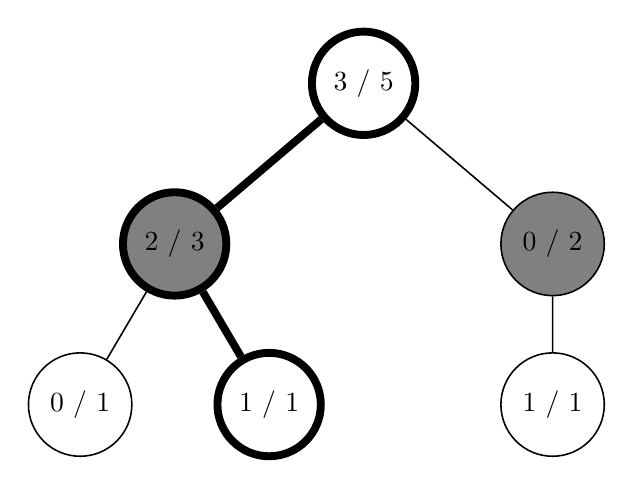
\begin{tikzpicture}[bold, scale=12]
                % The Tree
                \node(0)[max]{3 / 5}
                child{node[min]{2 / 3}
                    child{node[max, thin]{0 / 1} edge from parent[thin]}
                    child{node[max]{1 / 1}}
                }
                child{[thin]node[min]{0 / 2}
                    child{node[max]{1 / 1}}
                };
            \end{tikzpicture}
        }
        \caption*{Selection}
    \end{subfigure}
    &
    \begin{subfigure}[b]{0.4\textwidth}
        \centering
        \resizebox{\textwidth}{!}{
            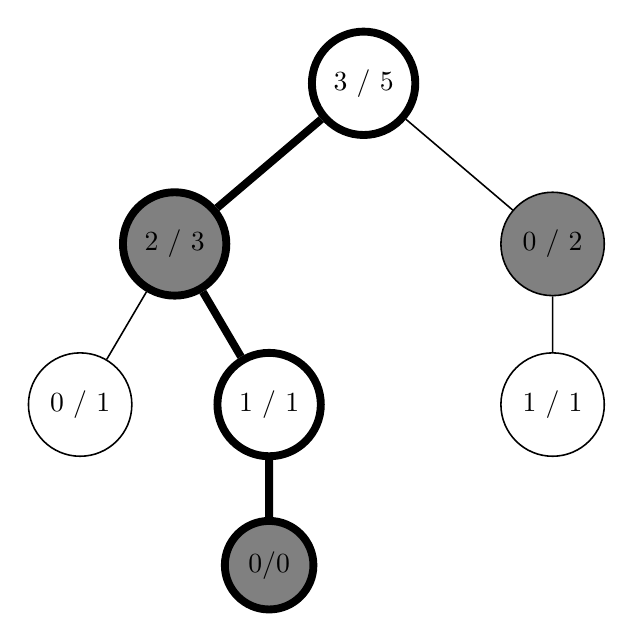
\begin{tikzpicture}[bold, scale=12]
                % The Tree
                \node(0)[max]{3 / 5}
                child{node[min]{2 / 3}
                    child{node[max, thin]{0 / 1} edge from parent[thin]}
                    child{node[max]{1 / 1}
                        child{node[min]{0/0}}
                    }
                }
                child{[thin]node[min]{0 / 2}
                    child{node[max]{1 / 1}}
                };
            \end{tikzpicture}
        }
        \caption*{Expansion}
    \end{subfigure}
    \\
    \begin{subfigure}[b]{0.4\textwidth}
        \centering
        \resizebox{\textwidth}{!}{
            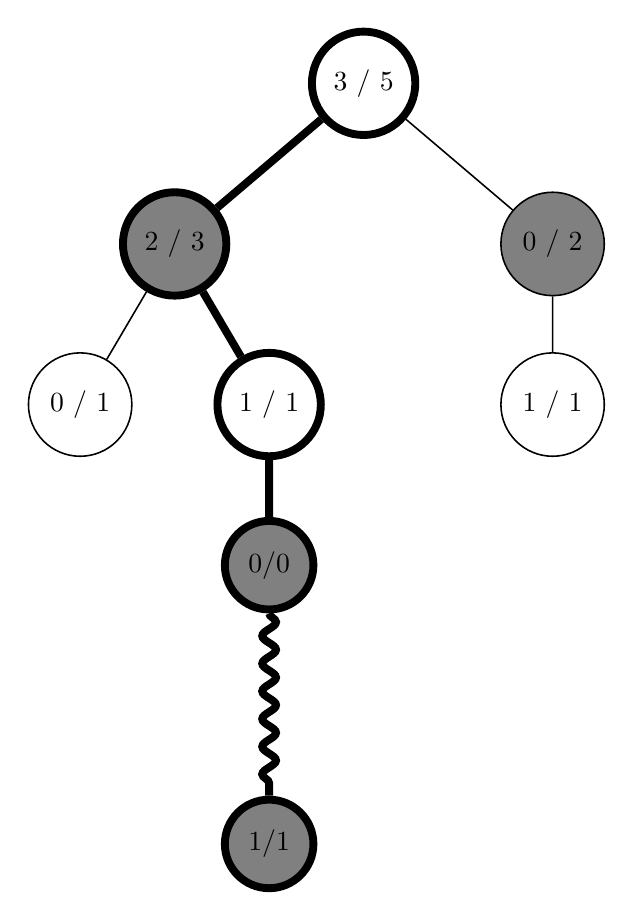
\begin{tikzpicture}[bold, scale=12]
                % The Tree
                \node(0)[max]{3 / 5}
                child{node[min]{2 / 3}
                    child{node[max, thin]{0 / 1} edge from parent[thin]}
                    child{node[max]{1 / 1}
                        child{node[min]{0/0}
                            child{node[min, yshift=-1.5cm]{1/1} edge from parent[decorate, decoration=snake]}
                        }
                    }                }
                child{[thin]node[min]{0 / 2}
                    child{node[max]{1 / 1}}
                };
            \end{tikzpicture}
        }
        \caption*{Simulation}
    \end{subfigure}
    &
    \begin{subfigure}[b]{0.4\textwidth}
        \centering
        \resizebox{\textwidth}{!}{
            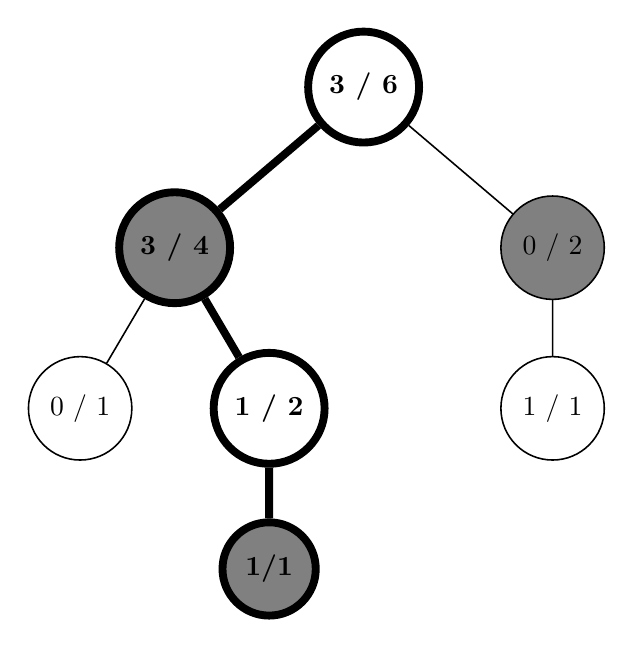
\begin{tikzpicture}[bold, scale=12]
                % The Tree
                \node(0)[max]{\textbf{3 / 6}}
                child{node[min]{\textbf{3 / 4}}
                    child{node[max, thin]{0 / 1} edge from parent[thin]}
                    child{node[max]{\textbf{1 / 2}}
                        child{node[min]{\textbf{1/1}}}
                    }
                }
                child{[thin]node[min]{0 / 2}
                    child{node[max]{1 / 1}}
                };
            \end{tikzpicture}
        }
        \caption*{Backpropagation}
    \end{subfigure}

    \end{tabular}


   
    \caption{}
    \label{fig:mcts_illustrated}

\end{figure}
